


\tikzset{every picture/.style={line width=0.75pt}} %set default line width to 0.75pt        

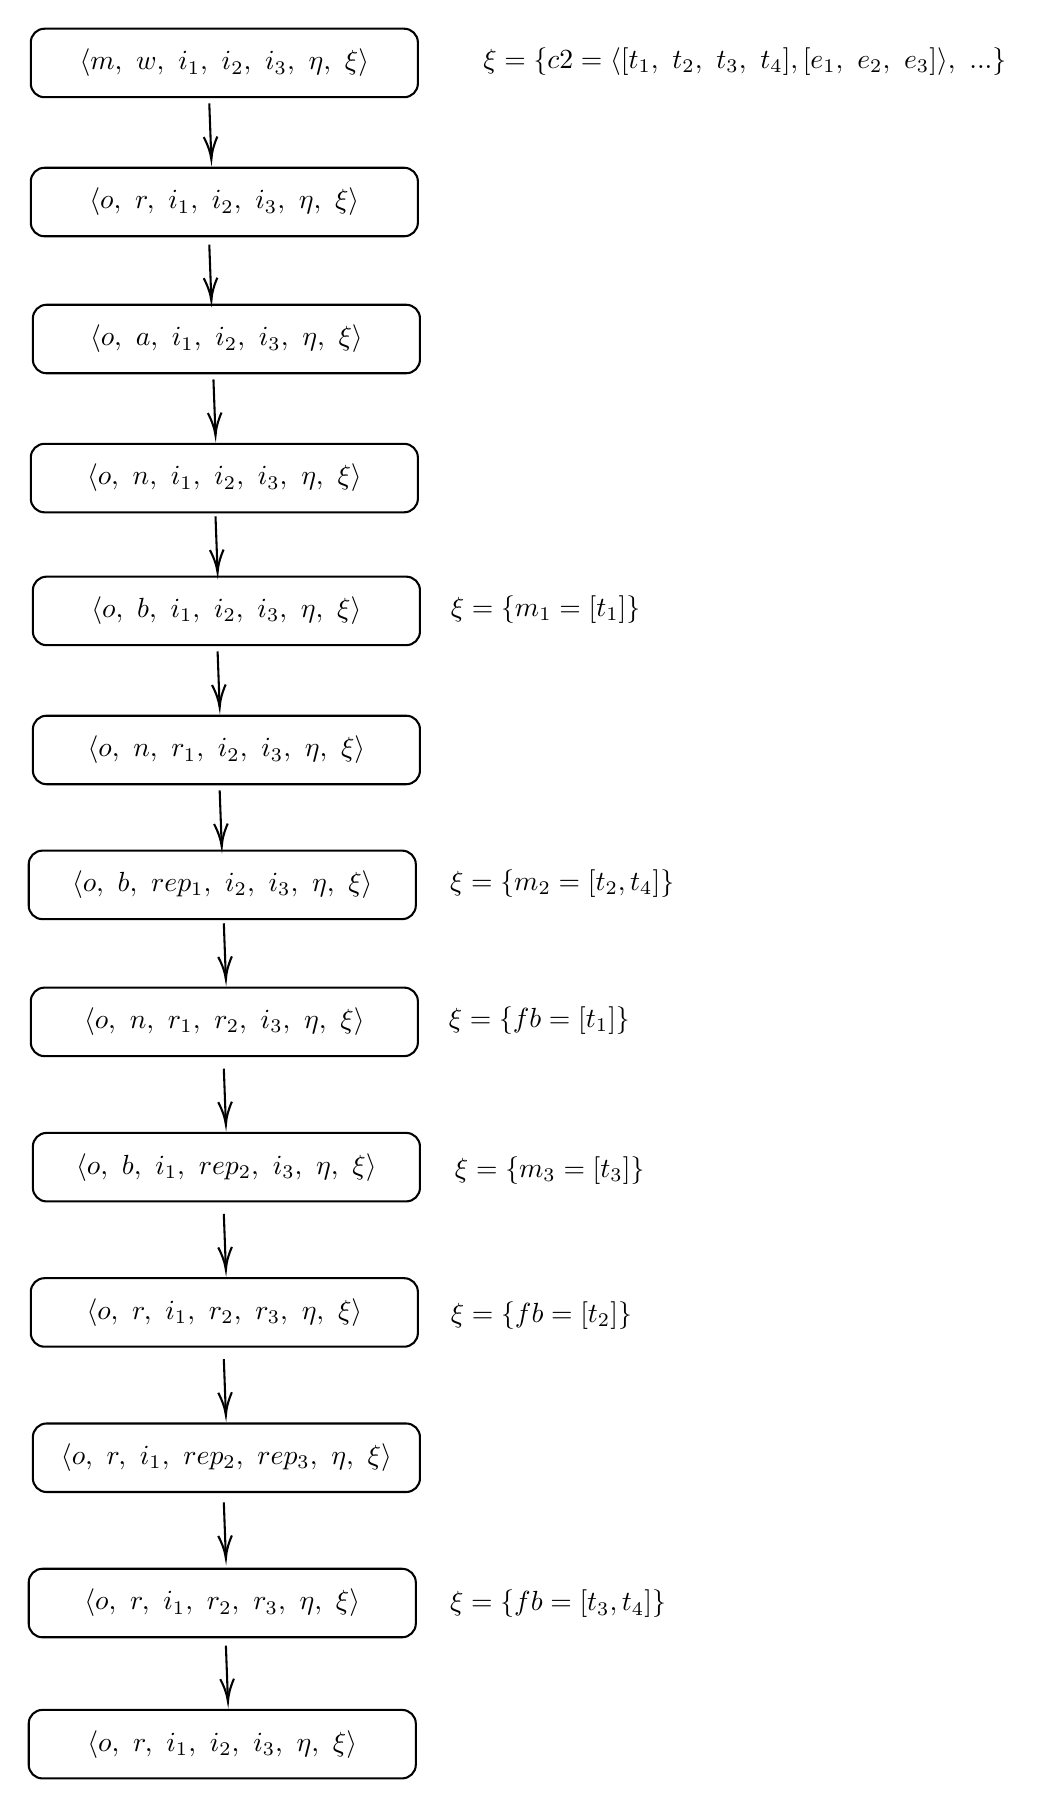
\begin{tikzpicture}[x=0.75pt,y=0.75pt,yscale=-1,xscale=1]
%uncomment if require: \path (0,865); %set diagram left start at 0, and has height of 865

%Rounded Rect [id:dp9048297129007524] 
\draw   (19,13.6) .. controls (19,9.95) and (21.95,7) .. (25.6,7) -- (198.9,7) .. controls (202.55,7) and (205.5,9.95) .. (205.5,13.6) -- (205.5,33.4) .. controls (205.5,37.05) and (202.55,40) .. (198.9,40) -- (25.6,40) .. controls (21.95,40) and (19,37.05) .. (19,33.4) -- cycle ;
%Rounded Rect [id:dp8152798292363221] 
\draw   (19,80.6) .. controls (19,76.95) and (21.95,74) .. (25.6,74) -- (198.9,74) .. controls (202.55,74) and (205.5,76.95) .. (205.5,80.6) -- (205.5,100.4) .. controls (205.5,104.05) and (202.55,107) .. (198.9,107) -- (25.6,107) .. controls (21.95,107) and (19,104.05) .. (19,100.4) -- cycle ;
%Rounded Rect [id:dp2611238064001401] 
\draw   (20,146.6) .. controls (20,142.95) and (22.95,140) .. (26.6,140) -- (199.9,140) .. controls (203.55,140) and (206.5,142.95) .. (206.5,146.6) -- (206.5,166.4) .. controls (206.5,170.05) and (203.55,173) .. (199.9,173) -- (26.6,173) .. controls (22.95,173) and (20,170.05) .. (20,166.4) -- cycle ;
%Rounded Rect [id:dp5474323622335151] 
\draw   (19,213.6) .. controls (19,209.95) and (21.95,207) .. (25.6,207) -- (198.9,207) .. controls (202.55,207) and (205.5,209.95) .. (205.5,213.6) -- (205.5,233.4) .. controls (205.5,237.05) and (202.55,240) .. (198.9,240) -- (25.6,240) .. controls (21.95,240) and (19,237.05) .. (19,233.4) -- cycle ;
%Rounded Rect [id:dp617967347556163] 
\draw   (20,277.6) .. controls (20,273.95) and (22.95,271) .. (26.6,271) -- (199.9,271) .. controls (203.55,271) and (206.5,273.95) .. (206.5,277.6) -- (206.5,297.4) .. controls (206.5,301.05) and (203.55,304) .. (199.9,304) -- (26.6,304) .. controls (22.95,304) and (20,301.05) .. (20,297.4) -- cycle ;
%Rounded Rect [id:dp6526355611328125] 
\draw   (20,344.6) .. controls (20,340.95) and (22.95,338) .. (26.6,338) -- (199.9,338) .. controls (203.55,338) and (206.5,340.95) .. (206.5,344.6) -- (206.5,364.4) .. controls (206.5,368.05) and (203.55,371) .. (199.9,371) -- (26.6,371) .. controls (22.95,371) and (20,368.05) .. (20,364.4) -- cycle ;
%Rounded Rect [id:dp6698610095556133] 
\draw   (18,409.6) .. controls (18,405.95) and (20.95,403) .. (24.6,403) -- (197.9,403) .. controls (201.55,403) and (204.5,405.95) .. (204.5,409.6) -- (204.5,429.4) .. controls (204.5,433.05) and (201.55,436) .. (197.9,436) -- (24.6,436) .. controls (20.95,436) and (18,433.05) .. (18,429.4) -- cycle ;
%Rounded Rect [id:dp9742586895494759] 
\draw   (19,475.6) .. controls (19,471.95) and (21.95,469) .. (25.6,469) -- (198.9,469) .. controls (202.55,469) and (205.5,471.95) .. (205.5,475.6) -- (205.5,495.4) .. controls (205.5,499.05) and (202.55,502) .. (198.9,502) -- (25.6,502) .. controls (21.95,502) and (19,499.05) .. (19,495.4) -- cycle ;
%Rounded Rect [id:dp34832491140564725] 
\draw   (20,545.6) .. controls (20,541.95) and (22.95,539) .. (26.6,539) -- (199.9,539) .. controls (203.55,539) and (206.5,541.95) .. (206.5,545.6) -- (206.5,565.4) .. controls (206.5,569.05) and (203.55,572) .. (199.9,572) -- (26.6,572) .. controls (22.95,572) and (20,569.05) .. (20,565.4) -- cycle ;
%Rounded Rect [id:dp07632153248409779] 
\draw   (19,615.6) .. controls (19,611.95) and (21.95,609) .. (25.6,609) -- (198.9,609) .. controls (202.55,609) and (205.5,611.95) .. (205.5,615.6) -- (205.5,635.4) .. controls (205.5,639.05) and (202.55,642) .. (198.9,642) -- (25.6,642) .. controls (21.95,642) and (19,639.05) .. (19,635.4) -- cycle ;
%Rounded Rect [id:dp38638906596830014] 
\draw   (20,685.6) .. controls (20,681.95) and (22.95,679) .. (26.6,679) -- (199.9,679) .. controls (203.55,679) and (206.5,681.95) .. (206.5,685.6) -- (206.5,705.4) .. controls (206.5,709.05) and (203.55,712) .. (199.9,712) -- (26.6,712) .. controls (22.95,712) and (20,709.05) .. (20,705.4) -- cycle ;
%Rounded Rect [id:dp2961818663412775] 
\draw   (18,755.6) .. controls (18,751.95) and (20.95,749) .. (24.6,749) -- (197.9,749) .. controls (201.55,749) and (204.5,751.95) .. (204.5,755.6) -- (204.5,775.4) .. controls (204.5,779.05) and (201.55,782) .. (197.9,782) -- (24.6,782) .. controls (20.95,782) and (18,779.05) .. (18,775.4) -- cycle ;
%Rounded Rect [id:dp1419509373702863] 
\draw   (18,823.6) .. controls (18,819.95) and (20.95,817) .. (24.6,817) -- (197.9,817) .. controls (201.55,817) and (204.5,819.95) .. (204.5,823.6) -- (204.5,843.4) .. controls (204.5,847.05) and (201.55,850) .. (197.9,850) -- (24.6,850) .. controls (20.95,850) and (18,847.05) .. (18,843.4) -- cycle ;
%Straight Lines [id:da25623652531692265] 
\draw    (105,43) -- (105.93,68) ;
\draw [shift={(106,70)}, rotate = 267.88] [color={rgb, 255:red, 0; green, 0; blue, 0 }  ][line width=0.75]    (10.93,-3.29) .. controls (6.95,-1.4) and (3.31,-0.3) .. (0,0) .. controls (3.31,0.3) and (6.95,1.4) .. (10.93,3.29)   ;
%Straight Lines [id:da9454848916406987] 
\draw    (105,111) -- (105.93,136) ;
\draw [shift={(106,138)}, rotate = 267.88] [color={rgb, 255:red, 0; green, 0; blue, 0 }  ][line width=0.75]    (10.93,-3.29) .. controls (6.95,-1.4) and (3.31,-0.3) .. (0,0) .. controls (3.31,0.3) and (6.95,1.4) .. (10.93,3.29)   ;
%Straight Lines [id:da9308850791504091] 
\draw    (107,176) -- (107.93,201) ;
\draw [shift={(108,203)}, rotate = 267.88] [color={rgb, 255:red, 0; green, 0; blue, 0 }  ][line width=0.75]    (10.93,-3.29) .. controls (6.95,-1.4) and (3.31,-0.3) .. (0,0) .. controls (3.31,0.3) and (6.95,1.4) .. (10.93,3.29)   ;
%Straight Lines [id:da6987828125639035] 
\draw    (108,242) -- (108.93,267) ;
\draw [shift={(109,269)}, rotate = 267.88] [color={rgb, 255:red, 0; green, 0; blue, 0 }  ][line width=0.75]    (10.93,-3.29) .. controls (6.95,-1.4) and (3.31,-0.3) .. (0,0) .. controls (3.31,0.3) and (6.95,1.4) .. (10.93,3.29)   ;
%Straight Lines [id:da38465000460546606] 
\draw    (109,307) -- (109.93,332) ;
\draw [shift={(110,334)}, rotate = 267.88] [color={rgb, 255:red, 0; green, 0; blue, 0 }  ][line width=0.75]    (10.93,-3.29) .. controls (6.95,-1.4) and (3.31,-0.3) .. (0,0) .. controls (3.31,0.3) and (6.95,1.4) .. (10.93,3.29)   ;
%Straight Lines [id:da7402304756808019] 
\draw    (110,374) -- (110.93,399) ;
\draw [shift={(111,401)}, rotate = 267.88] [color={rgb, 255:red, 0; green, 0; blue, 0 }  ][line width=0.75]    (10.93,-3.29) .. controls (6.95,-1.4) and (3.31,-0.3) .. (0,0) .. controls (3.31,0.3) and (6.95,1.4) .. (10.93,3.29)   ;
%Straight Lines [id:da32843301316145035] 
\draw    (112,438) -- (112.93,463) ;
\draw [shift={(113,465)}, rotate = 267.88] [color={rgb, 255:red, 0; green, 0; blue, 0 }  ][line width=0.75]    (10.93,-3.29) .. controls (6.95,-1.4) and (3.31,-0.3) .. (0,0) .. controls (3.31,0.3) and (6.95,1.4) .. (10.93,3.29)   ;
%Straight Lines [id:da33931279270538006] 
\draw    (112,508) -- (112.93,533) ;
\draw [shift={(113,535)}, rotate = 267.88] [color={rgb, 255:red, 0; green, 0; blue, 0 }  ][line width=0.75]    (10.93,-3.29) .. controls (6.95,-1.4) and (3.31,-0.3) .. (0,0) .. controls (3.31,0.3) and (6.95,1.4) .. (10.93,3.29)   ;
%Straight Lines [id:da4793309632596934] 
\draw    (112,578) -- (112.93,603) ;
\draw [shift={(113,605)}, rotate = 267.88] [color={rgb, 255:red, 0; green, 0; blue, 0 }  ][line width=0.75]    (10.93,-3.29) .. controls (6.95,-1.4) and (3.31,-0.3) .. (0,0) .. controls (3.31,0.3) and (6.95,1.4) .. (10.93,3.29)   ;
%Straight Lines [id:da7517013161282193] 
\draw    (112,648) -- (112.93,673) ;
\draw [shift={(113,675)}, rotate = 267.88] [color={rgb, 255:red, 0; green, 0; blue, 0 }  ][line width=0.75]    (10.93,-3.29) .. controls (6.95,-1.4) and (3.31,-0.3) .. (0,0) .. controls (3.31,0.3) and (6.95,1.4) .. (10.93,3.29)   ;
%Straight Lines [id:da06264248753342316] 
\draw    (112,717) -- (112.93,742) ;
\draw [shift={(113,744)}, rotate = 267.88] [color={rgb, 255:red, 0; green, 0; blue, 0 }  ][line width=0.75]    (10.93,-3.29) .. controls (6.95,-1.4) and (3.31,-0.3) .. (0,0) .. controls (3.31,0.3) and (6.95,1.4) .. (10.93,3.29)   ;
%Straight Lines [id:da8026456818678067] 
\draw    (113,786) -- (113.93,811) ;
\draw [shift={(114,813)}, rotate = 267.88] [color={rgb, 255:red, 0; green, 0; blue, 0 }  ][line width=0.75]    (10.93,-3.29) .. controls (6.95,-1.4) and (3.31,-0.3) .. (0,0) .. controls (3.31,0.3) and (6.95,1.4) .. (10.93,3.29)   ;

% Text Node
\draw (112.25,23.5) node    {$\langle m,\ w,\ i_{1} ,\ i_{2} ,\ i_{3} ,\ \eta ,\ \xi \rangle $};
% Text Node
\draw (112.25,90.5) node    {$\langle o,\ r,\ i_{1} ,\ i_{2} ,\ i_{3} ,\ \eta ,\ \xi \rangle $};
% Text Node
\draw (363,23) node    {$\xi =\{c2=\langle [ t_{1} ,\ t_{2} ,\ t_{3} ,\ t_{4}] ,[ e_{1} ,\ e_{2} ,\ e_{3}] \rangle ,\ ...\}$};
% Text Node
\draw (113.25,156.5) node    {$\langle o,\ a,\ i_{1} ,\ i_{2} ,\ i_{3} ,\ \eta ,\ \xi \rangle $};
% Text Node
\draw (112.25,223.5) node    {$\langle o,\ n,\ i_{1} ,\ i_{2} ,\ i_{3} ,\ \eta ,\ \xi \rangle $};
% Text Node
\draw (113.25,287.5) node    {$\langle o,\ b,\ i_{1} ,\ i_{2} ,\ i_{3} ,\ \eta ,\ \xi \rangle $};
% Text Node
\draw (267,287) node    {$\xi =\{m_{1} =[ t_{1}]\}$};
% Text Node
\draw (113.25,354.5) node    {$\langle o,\ n,\ r_{1} ,\ i_{2} ,\ i_{3} ,\ \eta ,\ \xi \rangle $};
% Text Node
\draw (111.25,419.5) node    {$\langle o,\ b,\ rep_{1} ,\ i_{2} ,\ i_{3} ,\ \eta ,\ \xi \rangle $};
% Text Node
\draw (275,419) node    {$\xi =\{m_{2} =[ t_{2} ,t_{4}]\}$};
% Text Node
\draw (112.25,485.5) node    {$\langle o,\ n,\ r_{1} ,\ r_{2} ,\ i_{3} ,\ \eta ,\ \xi \rangle $};
% Text Node
\draw (113.25,555.5) node    {$\langle o,\ b,\ i_{1} ,\ rep_{2} ,\ i_{3} ,\ \eta ,\ \xi \rangle $};
% Text Node
\draw (269,557) node    {$\xi =\{m_{3} =[ t_{3}]\}$};
% Text Node
\draw (112.25,625.5) node    {$\langle o,\ r,\ i_{1} ,\ r_{2} ,\ r_{3} ,\ \eta ,\ \xi \rangle $};
% Text Node
\draw (113.25,695.5) node    {$\langle o,\ r,\ i_{1} ,\ rep_{2} ,\ rep_{3} ,\ \eta ,\ \xi \rangle $};
% Text Node
\draw (111.25,765.5) node    {$\langle o,\ r,\ i_{1} ,\ r_{2} ,\ r_{3} ,\ \eta ,\ \xi \rangle $};
% Text Node
\draw (111.25,833.5) node    {$\langle o,\ r,\ i_{1} ,\ i_{2} ,\ i_{3} ,\ \eta ,\ \xi \rangle $};
% Text Node
\draw (265,627) node    {$\xi =\{fb=[ t_{2}]\}$};
% Text Node
\draw (264,485) node    {$\xi =\{fb=[ t_{1}]\}$};
% Text Node
\draw (273,766) node    {$\xi =\{fb=[ t_{3} ,t_{4}]\}$};


\end{tikzpicture}